% ARTICLE 2 ----
% This is just here so I know exactly what I'm looking at in Rstudio when messing with stuff.
% Options for packages loaded elsewhere
\PassOptionsToPackage{unicode}{hyperref}
\PassOptionsToPackage{hyphens}{url}
%
\documentclass[
  11pt,
]{article}
\usepackage{lmodern}
\usepackage{amssymb,amsmath}
\usepackage{ifxetex,ifluatex}
\ifnum 0\ifxetex 1\fi\ifluatex 1\fi=0 % if pdftex
  \usepackage[T1]{fontenc}
  \usepackage[utf8]{inputenc}
  \usepackage{textcomp} % provide euro and other symbols
\else % if luatex or xetex
  \usepackage{unicode-math}
  \defaultfontfeatures{Scale=MatchLowercase}
  \defaultfontfeatures[\rmfamily]{Ligatures=TeX,Scale=1}
\fi
% Use upquote if available, for straight quotes in verbatim environments
\IfFileExists{upquote.sty}{\usepackage{upquote}}{}
\IfFileExists{microtype.sty}{% use microtype if available
  \usepackage[]{microtype}
  \UseMicrotypeSet[protrusion]{basicmath} % disable protrusion for tt fonts
}{}
\makeatletter
\@ifundefined{KOMAClassName}{% if non-KOMA class
  \IfFileExists{parskip.sty}{%
    \usepackage{parskip}
  }{% else
    \setlength{\parindent}{0pt}
    \setlength{\parskip}{6pt plus 2pt minus 1pt}
    }
}{% if KOMA class
  \KOMAoptions{parskip=half}}
\makeatother
\usepackage{xcolor}
\IfFileExists{xurl.sty}{\usepackage{xurl}}{} % add URL line breaks if available
\urlstyle{same} % disable monospaced font for URLs
\usepackage[margin=1in]{geometry}
\usepackage{longtable,booktabs}
% Correct order of tables after \paragraph or \subparagraph
\usepackage{etoolbox}
\makeatletter
\patchcmd\longtable{\par}{\if@noskipsec\mbox{}\fi\par}{}{}
\makeatother
% Allow footnotes in longtable head/foot
\IfFileExists{footnotehyper.sty}{\usepackage{footnotehyper}}{\usepackage{footnote}}
\makesavenoteenv{longtable}
\usepackage{graphicx}
\makeatletter
\def\maxwidth{\ifdim\Gin@nat@width>\linewidth\linewidth\else\Gin@nat@width\fi}
\def\maxheight{\ifdim\Gin@nat@height>\textheight\textheight\else\Gin@nat@height\fi}
\makeatother
% Scale images if necessary, so that they will not overflow the page
% margins by default, and it is still possible to overwrite the defaults
% using explicit options in \includegraphics[width, height, ...]{}
\setkeys{Gin}{width=\maxwidth,height=\maxheight,keepaspectratio}
% Set default figure placement to htbp
\makeatletter
\def\fps@figure{htbp}
\makeatother
\setlength{\emergencystretch}{3em} % prevent overfull lines
\providecommand{\tightlist}{%
  \setlength{\itemsep}{0pt}\setlength{\parskip}{0pt}}
\setcounter{secnumdepth}{5}

\ifluatex
  \usepackage{selnolig}  % disable illegal ligatures
\fi
\newlength{\cslhangindent}
\setlength{\cslhangindent}{1.5em}
\newlength{\csllabelwidth}
\setlength{\csllabelwidth}{3em}
\newenvironment{CSLReferences}[2] % #1 hanging-ident, #2 entry spacing
 {% don't indent paragraphs
  \setlength{\parindent}{0pt}
  % turn on hanging indent if param 1 is 1
  \ifodd #1 \everypar{\setlength{\hangindent}{\cslhangindent}}\ignorespaces\fi
  % set entry spacing
  \ifnum #2 > 0
  \setlength{\parskip}{#2\baselineskip}
  \fi
 }%
 {}
\usepackage{calc}
\newcommand{\CSLBlock}[1]{#1\hfill\break}
\newcommand{\CSLLeftMargin}[1]{\parbox[t]{\csllabelwidth}{#1}}
\newcommand{\CSLRightInline}[1]{\parbox[t]{\linewidth - \csllabelwidth}{#1}\break}
\newcommand{\CSLIndent}[1]{\hspace{\cslhangindent}#1}


\title{Disagreement and dissent on a bench: a quantitative empirical
analysis of the Czech Constitutional Court}
\author{true \and true}
\date{October 08, 2023}

% Jesus, okay, everything above this comment is default Pandoc LaTeX template. -----
% ----------------------------------------------------------------------------------
% I think I had assumed beamer and LaTex were somehow different templates.


\usepackage{kantlipsum}

\usepackage{abstract}
\renewcommand{\abstractname}{}    % clear the title
\renewcommand{\absnamepos}{empty} % originally center

\renewenvironment{abstract}
 {{%
    \setlength{\leftmargin}{0mm}
    \setlength{\rightmargin}{\leftmargin}%
  }%
  \relax}
 {\endlist}

\makeatletter
\def\@maketitle{%
  \newpage
%  \null
%  \vskip 2em%
%  \begin{center}%
  \let \footnote \thanks
      {\fontsize{18}{20}\selectfont\raggedright  \setlength{\parindent}{0pt} \@title \par}
    }
%\fi
\makeatother


\title{Disagreement and dissent on a bench: a quantitative empirical
analysis of the Czech Constitutional Court }

\date{}

\usepackage{titlesec}

% 
\titleformat*{\section}{\large\bfseries}
\titleformat*{\subsection}{\normalsize\itshape} % \small\uppercase
\titleformat*{\subsubsection}{\normalsize\itshape}
\titleformat*{\paragraph}{\normalsize\itshape}
\titleformat*{\subparagraph}{\normalsize\itshape}

% add some other packages ----------

% \usepackage{multicol}
% This should regulate where figures float
% See: https://tex.stackexchange.com/questions/2275/keeping-tables-figures-close-to-where-they-are-mentioned
\usepackage[section]{placeins}



\makeatletter
\@ifpackageloaded{hyperref}{}{%
\ifxetex
  \PassOptionsToPackage{hyphens}{url}\usepackage[setpagesize=false, % page size defined by xetex
              unicode=false, % unicode breaks when used with xetex
              xetex]{hyperref}
\else
  \PassOptionsToPackage{hyphens}{url}\usepackage[draft,unicode=true]{hyperref}
\fi
}

\@ifpackageloaded{color}{
    \PassOptionsToPackage{usenames,dvipsnames}{color}
}{%
    \usepackage[usenames,dvipsnames]{color}
}
\makeatother
\hypersetup{breaklinks=true,
            bookmarks=true,
            pdfauthor={Author 1 () and Author 2 ()},
             pdfkeywords = {empirical legal research, courts, dissents,
judicial behavior, political science, Bayesian statistics, regression
analysis},
            pdftitle={Disagreement and dissent on a bench: a
quantitative empirical analysis of the Czech Constitutional Court},
            colorlinks=true,
            citecolor=blue,
            urlcolor=blue,
            linkcolor=magenta,
            pdfborder={0 0 0}}
\urlstyle{same}  % don't use monospace font for urls

% Add an option for endnotes. -----



% This will better treat References as a section when using natbib
% https://tex.stackexchange.com/questions/49962/bibliography-title-fontsize-problem-with-bibtex-and-the-natbib-package

% set default figure placement to htbp
\makeatletter
\def\fps@figure{htbp}
\makeatother



\usepackage{longtable}
\LTcapwidth=.95\textwidth
\linespread{1.05}
\usepackage{hyperref}
\usepackage{float}

\newtheorem{hypothesis}{Hypothesis}

\usepackage{setspace}

% trick for moving figures to back of document
% really wish we'd knock this shit off with moving tables/figures to back of document
% but, alas...

% 
% Optional code chunks ------
% SOURCE: https://stackoverflow.com/questions/50702942/does-rmarkdown-allow-captions-and-references-for-code-chunks



\begin{document}

% \textsf{\textbf{This is sans-serif bold text.}}
% \textbf{\textsf{This is bold sans-serif text.}}


% \maketitle

{% \usefont{T1}{pnc}{m}{n}
\setlength{\parindent}{0pt}
\thispagestyle{plain}
{%\fontsize{18}{20}\selectfont\raggedright
\maketitle  % title \par

}




{
   \vskip 13.5pt\relax \normalsize\fontsize{11}{12}
   \MakeUppercase{Author
1}, \small{}   \par \vskip -3.5pt \MakeUppercase{Author 2}, \small{}   

}

}








\begin{abstract}

%    \hbox{\vrule height .2pt width 39.14pc}

    \vskip 8.5pt % \small

\noindent \small{The decision of a judge to dissent or not to dissent
opens up avenue for strategical considerations. Building on the
economic-strategic account of judicial behavior developed by Lee
Epstein, Richard A. Posner and William M. Landes, we develop and test
multiple hyptotheses on the Czech Constitutional Court. To test the
hypotheses, we utilize Bayesian regression analyses. We find that the
workload of a judge does affect their dissenting behavior as previous
research in the US context suggests. We also find that a dissent imputes
substantial costs on the majority that produces longer arguments to
address a dissent, the effect being stronger the more disagreement there
is on the bench. Thirdly, we find that dissents bring about significant
collegiality costs to the dissenter. Lastly, we confirm the carry over
effect of alleged judicial coalitions formed in the plenary proceedings
to the 3-member panel proceedings. Simply put, CCC judges are more
likely to disagree when sitting on a bench with members from both
coalitions.}


\vskip 8.5pt \noindent \emph{Keywords}: empirical legal research,
courts, dissents, judicial behavior, political science, Bayesian
statistics, regression analysis \par

%    \hbox{\vrule height .2pt width 39.14pc}



\end{abstract}


\vskip -8.5pt


 % removetitleabstract


\setlength{\parindent}{16pt}
\setlength{\parskip}{0pt}

% We'll put doublespacing here
\doublespacing
% Remember to cut it out later before bib
\vspace{30pt}

\hypertarget{introduction}{%
\section{Introduction}\label{introduction}}

Empirical legal research has been slowly but surely finding it's outside
the predominant US context. Historically though most of the empirical
studies have been conducted in the US, especially the Supreme Court,
context (such as Boyd, Epstein, and Martin 2010; Carrubba et al. 2012;
Epstein, Landes, and Posner 2011). We now know that judgments are what
judges had for a breakfast. Put less pompously, there are many theories
and approaches for explanation of judicial behavior (Posner 2010). What
we do not know is the extent to which these theories and explanations
carry over to other legal systems and context.

In our article, we set out to conduct an empirical research into the
circumstances of disagreement on a court bench, more specifically
whether Czech constitutional justices behave strategically in when and
under what circumstances they dissent and whether there is an interplay
between the behavior at different institutional level within the Czech
Constitutional Court (``CCC'').

Our research is loosely inspired by a similar research by Epstein,
Landes, and Posner (2011), who studied under which circumstances do US
judges generally dissent. More specifically, they built a formal
economic model based on the strategic account of judicial behavior. In
particular, they tested the dependence of dissent rate on workload, the
dependence of dissent rate on size of courts, the dependence of dissent
rate on the ideological distance, and the dependence of length of
majority argumentation on the presence of a dissenting opinion. In our
study, we test our hypotheses adopted to the CCC context that are
nonetheless based on similar theoretical grounds.

We adapt the theories constructed in the US context to the civil law and
Czech judiciary contexts. We test whether the length of majority
argumentation depends on the presence of one or more dissents, whether
the workload of a judge affects their dissenting behavior, whether the
dissenting behavior of judges changes at the start and end of their
terms, and, lastly, whether relationships formed during the plenary
sessions, as posited by the Czech legal scholarship, carry over to
3-member panel proceedings.

We find that a dissent imputes costs on the majority that produces
longer arguments to address a dissent. The effect is stronger the more
disagreement there is on the bench. We find that the workload of a judge
does decrease the likelihood of dissent. Moreover, our analysis
corresponds to the theory that dissents bring about significant
collegiality costs for the dissenter. Lastly, we reveal similar trends
in behavior of judicial coalitions from plenary proceedings also in the
3-member panel proceedings.

Our article proceeds as follows. We start out with a theory. We explain
the main differences between the expectations based on the theory in the
CCC context in comparison to the SCOTUS context and based on that we
draw the hypotheses for the empirical part. We briefly explain the
choice of our broad methodological framework: the Bayesian statistics.
We proceed to test the hypotheses in empirical part divided into
sections one per each hypothesis. We discuss the pitfalls of our
research and potential room for improvement afterwards. Lastly, we
conclude with a summary of our findings.

\hypertarget{theory}{%
\section{Theory}\label{theory}}

In general, there are multiple accounts of behavior of judges'. The
first that had dominated until \textasciitilde the end of 20th century
posited that judges are policy oriented. A lot of research has been
conducted on whether, how and to what extent do judges indeed seek to
advance the policies they desire (Berdejó and Chen 2017; Clark and
Lauderdale 2010; Dworkin 1980; Kastellec 2016; Moyer and Tankersley
2012).

However, as of recently, the perspective on judges has shifted. Judges
are now allegedly strategic and rational actors. One of the early
pioneers of this approach Posner (1993) presents a simple model of
judicial utility as function mainly of income, leisure and judicial
voting. Further research followed the Posner mode and presented
alternative models of judicial utility (based on economic psychology
Foxall (2004)). Replacing the policy oriented approaches, which hold
judges to pursue political policy oriented goals, researchers now focus
more on their self-interest in terms of career progression, higher
income, or lesser workload (Carrubba et al. 2012; Epstein and Knight
2000). Posner (2010) presents nine theories of approach for judicial
behaviour, from which we mostly draw on the economical and sociological
theory. Economic theory of judicial behaviour treats the judges as a
rational, self-interested, utility maximizer and sociological theory of
judicial behaviour incorporates factors of strategic calculation,
emotion, and group polarization.

Epstein, Landes, and Posner (2011) based their theory of dissents on the
strategic-economic framework of self-interested strategically motivated
judges. They presume that judges ``leisure preferences, or,
equivalently, effort aversion, which they trade off against their desire
to have a good reputation and to express their legal and policy beliefs
and preferences (and by doing so perhaps influence law and policy) by
their vote, and by the judicial opinion explaining their vote, in the
cases they hear.'' The benefits of a dissenting opinion are the
potential to undermine the majority opinion when the dissent is
influential and the enhanced reputation that the judge enjoys. The
dissenting opinion may be cited in the future by other judges or
publicly analysed by legal scholars.

The theories they presume and hypotheses they test rest on this
framework: in the policy-oriented framework, it would not make sense to
expect judges to dissent less as their workload increases. They would
still seek a way to advance their political agenda and research has
shown that dissenting opinions usually correspond to exactly just that
(Clark and Lauderdale 2010). However, in the strategic account, the
higher the workload of a judge, the more pressing the effort costs of a
dissent. Similarly, if a dissenting opinion imputes costs on the
majority, we can theoretically expect it to respond to the dissent with
a more thorough or detailed argumentation in the majority opinion.

In our study, we are empirically verifying such theoretical presumptions
taken from the US context and transplanted to the context of the CCC.
There are obstacles that a researcher faces when conduct an original
US-inspired research design in European context.

Firstly, a major obstacle in conducting and carrying the US research
elsewhere is data availability. We narrow our object of analysis to the
CCC because there is the largest variation in the dissenting behavior
(unlike on the Supreme Administrative Court). While there is not yet a
full fledged dataset on the CCC (like the SCOTUS or CJEU Brekke et al.
2023), we have managed to build a complete dataset on the CCC, which
includes complete text corpus, metadata about cases and background
information of the judges. Typically for the US context, Epstein,
Landes, and Posner (2011) include in their analysis the ideological
distance between judges but they are far from the only ones (Berdejó and
Chen 2017; Boyd, Epstein, and Martin 2010; Carrubba et al. 2012; Clark
and Lauderdale 2010; Kastellec 2016; Segal et al. 1995). The ideological
distance serves as one of the explanatory variables for dissent
aversion. The measures of ideological position of judges mainly rely on
information about their voting behavior. Regrettably such information is
in continental legal systems typically not made public: the votes in
cases are kept secret. Therefore, it is near impossible to construct a
measure of the political position of judges without knowing how they
voted in each case.

Secondly, we utilize variation of different institutional settings
rather than a in between courts variation between SCOTUS and Federal
Courts. The CCC is structured so that it can either decide cases in
3-member panels or a plenary session. Moreover, we are able to use the
variation of a judge rapporteur. To apprehend the institutional
variation, we interpose a short section on the CCC institutional setup
and the difference in comparison to the SCOTUS, which has repercussions
on our theory.

The CCC consists of 15 judges: a Chairman, two Vice-chairmains and
twelve judges who are members of the permanent 3- member panels
consisting of three judges. The CCC justices are elected for 10 years
and the appointment process is akin to that of SCOTUS: the President
proposes a candidate that is confirmed by the Czech Senate.

The CCC is currently entering its fourth decade, having been established
in 1993, with 3 ``generations'' of judges having been rotated so far
with the fourth term of the CCC being just around the corner. Concerning
the institutional setup, the CCC can decide a case in two formations:
there are four 3-member panels and a plenum, which attracts procedurally
specified cases. Thus, the size of the deciding body varies within the
court. So does the type of cases that get assigned to either type of
body.

Regarding the specific theory and hypotheses we zero in on, Epstein,
Landes, and Posner (2011) find the strategic aspect of dissenting in how
a judge squares their decision to either dissent or to avert a dissent
based on the costs and benefits of a dissent. The authors claim that
``{[}s{]}ince writing a dissenting opinion requires effort, which is a
cost, a judge will not dissent unless he anticipates a benefit from
dissenting that offsets his cost.'' The majority also accrues costs from
dissenting. In their words: ``{[}d{]}issenting imposes an effort cost on
the majority as well and sometimes a reputation cost too, if the
dissenting opinion criticizes the majority force- fully. To minimize the
dissenter's criticisms and retain the vote of the other judge in the
majority (in a panel of three judges, the normal number of judges who
decide a case in the federal courts of appeals), the author of the
majority opinion often will revise his opinion to meet, whether
explicitly or implicitly, the points made by the dissent.'' A following
hypotheses can be distilled:

H\textsubscript{1}: The presence of dissent positively affects the
length of the majority argumentation.

The room for the dissenting judge and the majority to address each other
differs between the two bodies. Based on our internal insight, there is
less back and forth interplay between the judges, more akin to the
SCOTUS context, and most of the communication is handled remotely in the
panel proceedings, whereas the plenum meets regularly to discuss the
cases in person. Despite that, procedurally speaking, the process of
generating dissents is the same. In both cases, the rapporteurs are
informed about the outcome of the vote, which is filed in the voting
record. The dissenting opinion is then sent to the judge rapporteur
before the decision is announced, as it cannot be added until after the
announcement. It is important to note that judges have the possibility,
not the obligation, to dissent. In other words, there is room for judges
to give way to strategic considerations.

To advance the theory further, what we believe that a presence of a
dissenting opinion truly captures is the expressed disagreement among
CCC judges. Since the individual cases are debated among the judges,
whether in person or remotely, it is possible to observe which side a
judge takes during the discussion before the final vote. The judges have
in either deciding body ample room to voice their disagreement, even if
they write the dissenting opinion last minute. There is no evidence that
would suggest otherwise - that the normal behavior would be to remain
silent until the vote and then present the majority with a dissenting
opinion.\footnote{We are aware of one judge whose behavior resembles the
  description, the rest voice their disagreement openly.} Thus,
technically speaking, the true explanatory variable of our theory is at
all times the varying disagreement among judges.

According to Epstein, Landes, and Posner (2011): ``{[}t{]}he economic
theory of judicial behavior predicts that a decline in the judicial
workload would lower the opportunity cost of dissenting and increase the
frequency of dissents, and also that the greater the ideological
heterogeneity among judges the more likely they are to disagree and so
the higher the dissent rate will be.'' The authors find a positive
relationship between the dissent rate, i.e., number of dissents divided
by the number of cases, and caseload. Our second hypothesis may be
formulated as

H\textsubscript{2}: The higher the workload of a judge, the lower their
likelihood of dissent.

Epstein, Landes, and Posner (2011) address the issue of collegiality
costs arising for a dissenting judge: ``The effort involved in these
revisions, and the resentment at criticism by the dissenting judge, may
impose a collegiality cost on the dissenting judge by making it more
difficult for him to persuade judges to join his majority opinions in
future cases.'' Based on this theory, they predict and indeed
empirically confirm that ``dissents will be less frequent in circuits
that have fewer judges because any two of its judges will sit together
more frequently and thus have a greater incentive to invest in
collegiality.'' Put simply, the researchers compare the dissent rates
between courts with differing number of members.

While it is hard for us to see how a variation between the number of
members in the plenary session and 3-member panels could be isolated
from a plethora of potential confounding variables, we are able to make
use of the limited term of CCC judges. We test whether judges that are
at the start of their term, and thus are aware that they will ``sit
together more frequently'' invest in collegiality by averting dissents
and whether when their term draws to an end, they give way to their
disagreement. This presumes that the outlook of sharing the 10 year term
with your colleagues at the beginning of judges' terms increases the
collegiality costs of dissenting, whereas at the end of their terms, the
collegiality costs decrease with the end of the shared term looming on
the horizon. We pose the research question, whether the judges'
likelihood of dissents varies across their terms as a result of
differing collegiality costs. We test third hypothesis:

H\textsubscript{3}: The judges are less likely to dissent at the
beginning of their dissents, whereas they are more likely to dissent at
the end of their terms.

Lastly, the research on judicial coalitions at the CCC has revealed that
the third period of CCC between 2013-2023 is rather polarized and that
there are two big coalitions of judges that clash against each other
(Chmel 2021; Smekal et al. 2021; Vartazaryan 2022). The articles rely
primarily on network analysis of the dissenting opinions in the plenary
proceedings and make inferential conclusions based on a rather
superficial descriptive analysis. We hypothesize that should the
relationship from the plenary sessions indeed exist, they should also
carry over to the 3-member panel hearings. Our hypothesis is that panels
composed of judges from both coalitions will be more likely to show
disagreement in the form of dissenting opinion. If this shows to be
true, it would provide further evidence to the two coalition theory of
the CCC (Chmel 2021; Vartazaryan 2022; Smekal et al. 2021). The Vyhnánek
article goes so far to coin the first coalition as a more left-leaning
and the second as a more right-leaning, whereas we are not convinced by
this label.

We test whether the presumable existence of the coalitions carry over to
and have any effect on the dissenting behavior of judges in the panels.
Consistent with our theoretical part, we believe that a dissenting
opinion reflects disagreement on the judicial bench. Our intuition
suggests that if indeed there are two coalitions in the plenary
proceedings, which strongly disagree between each other, such a
disagreement should, theoretically, carry over to the panel level. Our
research question is thus whether judicial coalitions formed in the
plenary proceedings affect the amount of disagreement and, in turn, the
likelihood of dissent of a judge in 3-member panels. Our hypothesis is
as follows:

H\textsubscript{4}: Having a 3-member panel composed of members of both
judicial coalitions increases judges' likelihood of a dissent.

\hypertarget{method}{%
\section{Method}\label{method}}

Methodologically, we rely on regression based research design with
observational data. Unfortunately, the legal environment does not lend
itself easily to (quasi)experimental design.

Our study deviates in that we utilize the \emph{Bayesian} rather than
\emph{frequentist} framework of statistics. Without delving too much
into the Bayesian versus frequentist statistics, we opt for the Bayesian
framework for it, we believe, reflects better our understanding of
probability and scientific inquiry.\footnote{We include a longer
  description of our reasoning in the appendix} There are two major
differences in understanding of concepts between the two approaches
towards statistics: that of role of prior knowledge and that of
probability. The Bayesian framework rather than measuring the
uncertainty about observed data (personified by the p-value) measures
the uncertainty of the parameters of interests, given the observed data
and our prior knowledge. In simple terms, the Bayesian statistician puts
into doubt their conclusions about parameters of a certain model, given
the observed data and their prior knowledge. Mathematically, the
uncertainty is reflected in the fact that the posterior parameters are
drawn from a posterior distribution of the model and are just an
approximation of thereof.

The Basian computations are implemented in the R programming language
and STAN software, connected via the RStan package and utilized within
the tidymodels framework. We include all the model specifications and
diagnoses in the appendix. In this article, we mainly focus on the
output of the models and the interpretation of thereof.

The Czech Apex Court dataset used for our analysis comprises the dataset
CCC decisions. The Czech Apex Court dataset includes complete database
of decisions of the CCC, SAC and the Czech Supreme Court, including
comprehensive metadata, text corpus, as well as additional information
mined from the texts or publicly available sources, such as case
references, compositions, or background information of the judges. The
analysis was limited up until the end of 2022. We filtered only those
decisions, where a variation in the dissenting behavior could
procedurally be observed: procedural decisions were filtered out as they
require unanimity among the judges and do not leave any space for
disagreement.

\hypertarget{model-specifications-and-results}{%
\section{Model specifications and
results}\label{model-specifications-and-results}}

\hypertarget{h1-effect-of-presence-of-dissenting-opinion-on-the-length-of-majority-argumentation}{%
\subsection{\texorpdfstring{H\textsubscript{1}: Effect of presence of
dissenting opinion on the length of majority
argumentation}{H1: Effect of presence of dissenting opinion on the length of majority argumentation}}\label{h1-effect-of-presence-of-dissenting-opinion-on-the-length-of-majority-argumentation}}

\hypertarget{model-specification}{%
\subsubsection{Model specification}\label{model-specification}}

In the original study, the authors collected roughly 446 SCOTUS and 1025
US court of appeals decisions. They then create regression models to see
whether the presence of at least one dissenting opinion affected the
length of the majority opinion. Based on application of their model to
the SCOTUS data, the trio of authors found a statistically significant
and positive relationship between presence of at least two dissenting
opinions and the length of the majority decision, as well as control
variable - the importance of the case. While we are aware that the
importance or salience of a case is probably the key confounding
variable, measuring as a post-treatment amount of references of that
decision might introduce further bias

\hypertarget{conceptualizing-importance-of-a-case-as-a-control-variable}{%
\paragraph{Conceptualizing importance of a case as a control
variable}\label{conceptualizing-importance-of-a-case-as-a-control-variable}}

In general, when utilizing a regression design with observational data,
as is our case, a researcher must satisfy certain conditions to be able
to interpret regression results as a causal relationship. The first is
the stable unit treatment value assumption (SUTVA) and the other is
usually referred to as \emph{conditional independence assumption}. This
condition requires that the assignment of treatment T to unit \emph{i}
is independent of any covariates \emph{X} of the unit \emph{i} that also
influence their outcome \emph{Y}. The CIA may be formalized as follows:

\[
{Y_{1i}, Y_{0i}} {\bot} T_{i}|X_{i}
\]

The notation follows the potential outcomes framework.
\{Y\textsubscript{1i}, Y\textsubscript{0i}\} refer to the outcome of a
unit i with or without treatment, in our case the presence of at least
one dissenting opinion. There are, in general, two types of causes of
bias: a confounding variable, which breaks the CIA, and reverse
causality. A confounding variable is such that

\begin{enumerate}
\def\labelenumi{(\arabic{enumi})}
\tightlist
\item
  has an effect on treatment status,
\item
  has an effect on the outcome over and above its effect on the
  treatment status.
\end{enumerate}

Not controlling for confounding variables causes an omitted variable
bias.

While at first glance it may thus seem that researchers should throw in
as many covariates as possible, that is in reality not the case. There
are examples of bad or unnecessary controls that are themselves an
outcome of the treatment (for a detailed discussion see Joshua D.
Angrist and Pischke 2009; Joshua David Angrist and Pischke 2015;
Montgomery, Nyhan, and Torres 2018). Among them are post-treatment
variables, which imply that all control variables must occur before the
treatment takes place.

We believe that importance of a decision is a potential confounding
variable as it clearly may impact both the length of a judgment as well
as the likelihood of a dissent. However, proxying it by the number of
citations in ensuing caselaw may present a bad post-treatment control
variable because it occurs and is measured after the decision to dissent
or not to dissent has been made. On top of the operationalization, we
are not exactly sure what kind of importance is being capture - is it
political or legal importance of a case? We presume that in our context,
it makes more sense to control for the complexity of case, we
nonetheless try to capture legal importance too. The \emph{formation of
the CCC} and the \emph{number of references to CCC caselaw} are better
pre-treatment proxies for the \emph{legal} importance and complexity of
a decision.

Institutionally, the CCC can decide cases either in 3-member panels or
in the whole plenary session. Put simply, we assume that more important
cases are decided in plenary rather than 3-member panel formation. The
plenary is more likely to rule on merits and its decisions are,
therefore, on average longer. Moreover, the dissent rate in the plenary
decisions is also higher. Thus, the formation of the CCC reflects the
importance of the case being decided, which has a confounding potential.

We confirm our intuition by comparing our metric of importance of a case
to Epstein's metric in the CCC context. While plenary decisions make up
only 1.5 \% of all CCC decisions, they make up 15 \% references in the
CCC caselaw. Unlike the Epstein metric, our metric is in any case
determined before the decision to dissent or not to dissent is made.
Thus, in our model, we're including a dummy variable for the formation
of a court, i.e., whether the decision was made in a 3 member panel or a
full court plenary.

Lastly, we wanted to address the complexity of a case. We believe it to
be another potential confounding variable: a more complex decision will
be undoubtably on average longer and it gives more room for disagreement
to arise. One way to measure complexity would be to how many legal
sources a legal decision refers. We presume that the number of
references to the Constitution, the main benchmark of the CCC's
constitutinal review, is rather invariable and does not necessarily
reflect complexity. A very complex case can pertain only one paragraph
of the very vaguely and abstractly drafted Constitution. Moreover, other
potential ways to measure complexity of a case would prove hard to
operationalize - such as the number of reviewed laws in the abstract
review. Because we could automatically identify all the self-references
within the CCC caselaw, we included the number of self-references in any
given CCC decision as a control variable for the complexity of a case.

Our final model thus looks as follows:

\[
W_{argument} = f(one\:dissent + more\:dissents + formation + number\:of\:selfreferences)
\] Building on the theory, in our model, we included the number of words
of the court argument part of a decision as the outcome variable.
Regarding the explanatory variables, we opted for (1) a dummy variable
signifying a presence of one dissent as an explanatory variable, (2) a
dummy variable signifying a presence of two or more dissents as an
explanatory variable, (3) the formation of the CCC as a control
variable, (4) the number of self-references. We code the one and two or
more dissents separately because we believe a higher number of dissents
implies a higher degree of disagreement. We lump the two and more
dissents into variable because the number of decisions with more than
two of dissents is few and far between.

\hypertarget{data-collection}{%
\subsubsection{Data collection}\label{data-collection}}

While the metadata of decisions contain information about a presence of
a dissenting opinion, regrettably, the CCC decisions are not neatly
split up like their SCOTUS counterparts. The text of the decision
contains both the majority opinion as well as the dissent without any
clear boundary from other parts of the structure. That is why we relied
on machine learning to extract the information about presence, position
of dissenting opinion as well as length of the majority argumentation in
the CCC decisions.

Utilizing machine learning unlocked one more avenue to further improve
the original model. Instead of conceptualizing the length of the
majority opinion as the whole majority opinion, we narrowed our inquiry
only to the majority argumentation rather than including, for example,
the heading or the facts of the case in the length of a majority opinion
variable. Therefore, we believe our model better reflects the
relationship between the presence of a dissent and the legal
argumentation of the majority.

To extract the length of dissents and length of majority argumentation,
multiple supervised classification algorithms were trained following
similar structure-mining attempts within the Czech context (Eliášek,
Kól, and Švaňa 2020; Harašta et al. 2019; and elsewhere Lüders and
Stohlman 2023). A sample of 200 decisions was manually annotated on a
paragraph level. The paragraphs were then represented either as dense
doc2vec vectors based on word2vec model of the whole CCC text corpus
(Mikolov et al. 2013) or as sparse document-term-matrix with the td-idf
values for each word. Positional encoding of a paragraph was added to
both representations of text. Because there was a large unbalance
between the classes, oversampling algorithm SMOTE was applied to balance
out the dataset, which is a standard practice when working with smaller
datasets (Fjelstul 2021).

Our classification followed in two stages. In the first step, the
dissenting opinions were classified from the rest of the decision so
that the positional encoding remained consistent across all cases.
Otherwise, in the decision without a dissenting opinion, usually a
conclusion or court argumentation was at the end of the decision,
whereas in the decisions with a dissent, the dissenting opinion was at
the end of the decision. That created confusion with the positional
encoding. Our first stage classification allowed us to separate the
dissenting opinion from the rest of the decision and then recalculate
the positional encoding for the remaining paragraphs. In the second
step, the remaining text as well as the decisions that did not contain a
dissenting opinion were classified into an inner structure consisting
of: (1) heading, (2) verdict, (3) procedure history, (4) complainant
arguments, (5) court arguments, (6) conclusion, (7) information on
further legal remedies, and (8) signature.

In line with the findings of Eliasek and Lüders articles, we tested and
compared three classification algorithms: - Support Vector Machines
(Gandhi 2018) with the sparse td-idf representation and Gradient Boosted
Decision Trees (Maklin 2019) and Random Forests with the dense doc2vec
embeddings. More complex algorithms did not provide any improvement in
accuracy at the cost of higher computing costs. The benchmark for both
classifiers was the zero rule, i.e., the proportion of the majority
class as a zero rule classifier would presume that all occurrences are
of that class and would be right the proportion amount of the time.

In the end, the XGBoost algorithm combined with the doc2vec embeddings
boasted the highest benchmark values (precision, accuracy, FScore). The
precision of the first stage classifier was \textasciitilde86 \%, above
the 75 \% zero rule benchmark. The precision of the second stage
classifier was \textasciitilde82 \%, well above the 37 \% zero rule
benchmark. Afterwards, both classification models were trained on all
annotated data and used to predict classes of the whole dataset.

\hypertarget{results}{%
\subsubsection{Results}\label{results}}

We opted for a completely pooled model as the data did not contain any
inherent structure (there were no clusters). We instead opted for the
Negative Binomial model, which allows for relaxing the assumption of
equality of variance of Y to its expected value in comparison to the
Poisson model. Thus, the explanatory variable, the number of words of
argumentation of the CCC \emph{Y}

\[
Y_{words} | \mu, r \sim NegBin(\mu, r)
\] As for the priors, we based the priors a cursory exploratory peak
into the data. All our priors follow a normal distribution, the
intercept being centered around the population mean. The remaining
priors were kept uninformative, because we simply have no previous
knowledge on the CCC. The negative binomial family employs a log link,
therefore the resulting estimates have to be interpreted as such. The
model did a resonable job of predicting the underlying data.

\vspace{10pt}

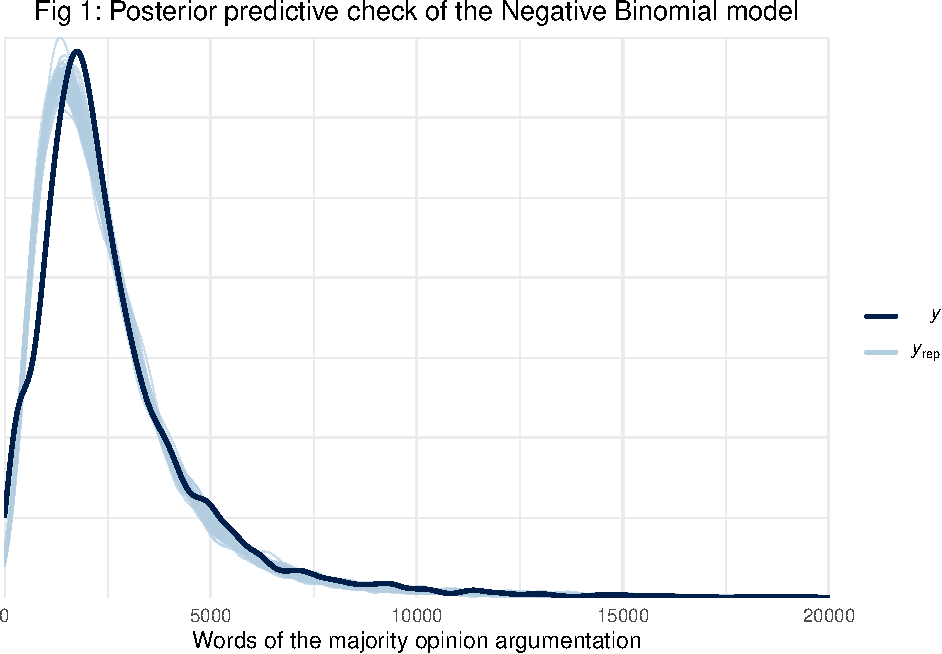
\includegraphics{dissents_article-anonymised_files/figure-latex/length_pp_check-1.pdf}

Parameters of both variables of interest are significantly different
from 0 as revealed by the density with 80 \% and 95 \% posterior
credible intervals.

\vspace{10pt}

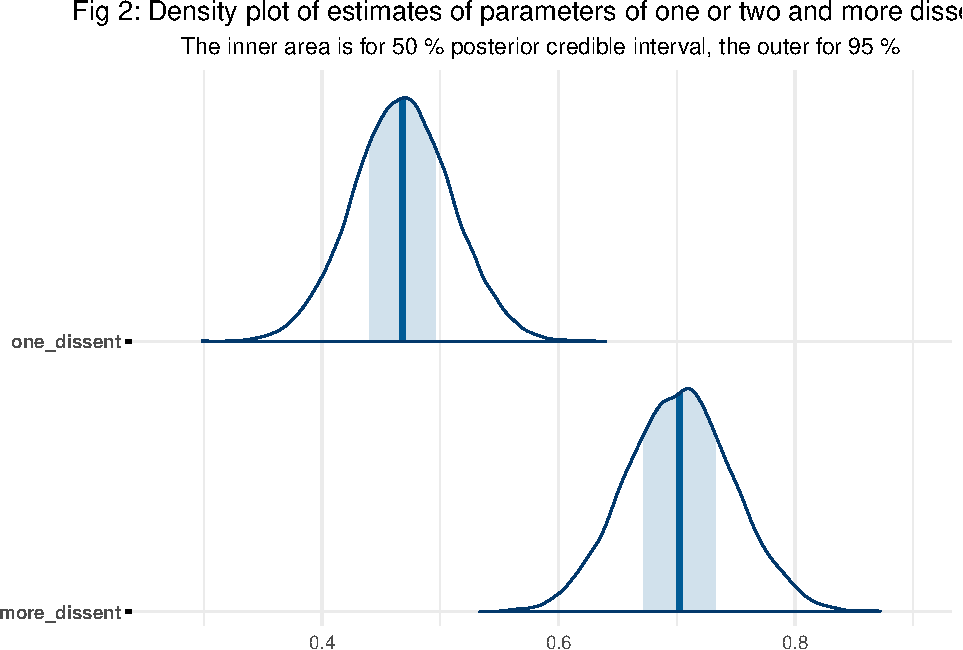
\includegraphics{dissents_article-anonymised_files/figure-latex/length_parameter_plots-1.pdf}

Even after controlling for all potential observable confounding
variables, the already unlogged regression table looks as follows

\begin{longtable}[]{@{}lrrrr@{}}
\toprule\noalign{}
term & estimate & std.error & conf.low & conf.high \\
\midrule\noalign{}
\endhead
\bottomrule\noalign{}
\endlastfoot
(Intercept) & 1869.63 & 1.01 & 1841.94 & 1897.17 \\
one\_dissent & 1.60 & 1.04 & 1.51 & 1.69 \\
more\_dissent & 2.02 & 1.05 & 1.90 & 2.14 \\
formationPlenum & 0.82 & 1.02 & 0.80 & 0.85 \\
n\_citations & 1.04 & 1.00 & 1.04 & 1.04 \\
\end{longtable}

In other words, the presence of one dissent implies an average
\emph{e}\textsuperscript{0.47} increase of words in the court arguments
part of judgment. Put in terms of percentage, a presence of one dissent
increases the length of the argumentation by 60 \%. The presence of two
or more dissents implies an average \emph{e}\textsuperscript{0.7}
increase of words in the court arguments part of judgment. That is a
staggering \textasciitilde100 \% increase in the length as a result of
presence of two or more dissenting opinions. To this end, the result of
our study is in line with the US study: a presence of dissenting opinion
increases the length of the majority opinion argumentation considerably.

We believe there are two potential ways to explain this behavior. Either
the majority simply takes the dissenting opinion seriously and addresses
the arguments raised in them or the presence of a dissenting opinion
reflects a deeper disagreement between judges that would have taken
place during the deliberation. Based on our knowledge of the inner
organisation of the court, the deeper disagreement explanation would fit
the plenary proceedings more accurately as a more thorough debate
usually takes place than in the 3-member panel proceedings. Such a
substantive explanation for our findings is supported by the fact that
decisions originating in the plenary proceedings are disproportionately
over-represented among decisions that contain at least one dissenting
opinion. This explanation is further supported by the larger effect of
having 2 or more dissents over just the 1 dissent. More dissenting
judges simply imply higher degree of disagreement on the bench. The
latter explanation fits within our theory of conceptualizing dissent as
a result of differing degree of disagreement on the bench. Be it as it
may, we conclude that a dissents imputes costs on the majority.

\hypertarget{h2-the-higher-the-workload-of-a-judge-the-lower-their-likelihood-of-dissent.}{%
\subsection{\texorpdfstring{H\textsubscript{2}: The higher the workload
of a judge, the lower their likelihood of
dissent.}{H2: The higher the workload of a judge, the lower their likelihood of dissent.}}\label{h2-the-higher-the-workload-of-a-judge-the-lower-their-likelihood-of-dissent.}}

\hypertarget{model-specification-1}{%
\subsubsection{Model specification}\label{model-specification-1}}

We could conceptualize the workload of a judge in multiple ways:

\begin{enumerate}
\def\labelenumi{\arabic{enumi}.}
\tightlist
\item
  the number of cases submitted and assigned to each judge rapporteur
  per year (we refer to this option as the caseload)
\item
  the number of unfinished cases as a judge rapporteur of any judge at
  the time of decision in any given decision (we refer to this option as
  workload), 3 and 4. as the yearly rate of change of thereof.
\end{enumerate}

The option 1 captures the caseload here is that of an individual judge
of decisions that they have to decide and write, or the rate of change
of thereof. The more cases the judges have to author each year, the
busier they are.

However, it is doubtful whether that is how a judge would perceive
workload. We believe our second measure captures the workload of a judge
better: the number of unfinished cases that any given judge has in the
moment of any given decision as a judge rapporteur. We firstly mined the
compositions of panels as well as the plenary from the text of the
decision. We then calculated the number of unfinished cases each judge
had at the time of any given decision as a judge rapporteur using the
date of submission and of decision of a case. We believe such a measure
captures the perceived workload of a judge much better: a judge knowing
that they have, for example, 20 in comparison to 100 decisions to draft
as a judge rapporteur is how they would perceive having had more
workload.

Similarly, instead of measuring dissent rate on the Constitutional court
in general, we can regress the number of dissents written by each judge
either per year on the caseload or we can regress the decision to
dissent of any given judge on their workload. Ideally, we would measure
both variables as rate of change. However, there are many observations
of the number of dissents with the value of 0. In these cases, the rate
of change would either be infinite or not a number (as a 0 would appear
either in the denominator or numerator of the rate of change formula).
Getting rid of the zeroes would imply a rather complex transformation
(for a more detailed overview of the possible transformations see
Hyndman 2010).

To address potential sources of bias in our regression analysis, we
consider the caseload of a judge to be assigned as good as random. The
cases once submitted to the CCC get assigned to individual judges based
on the alphabetic order of their surnames. There is no intentional case
selection in play. Therefore the assignment of the treatment, the
workload of a judge, is independent of other covariates and so is the
outcome of interest. The same applies to our last hypothesis. We include
time as a control variable because we observe that the workload of
judges increases over time and so does the number of dissents.

\vspace{10pt}

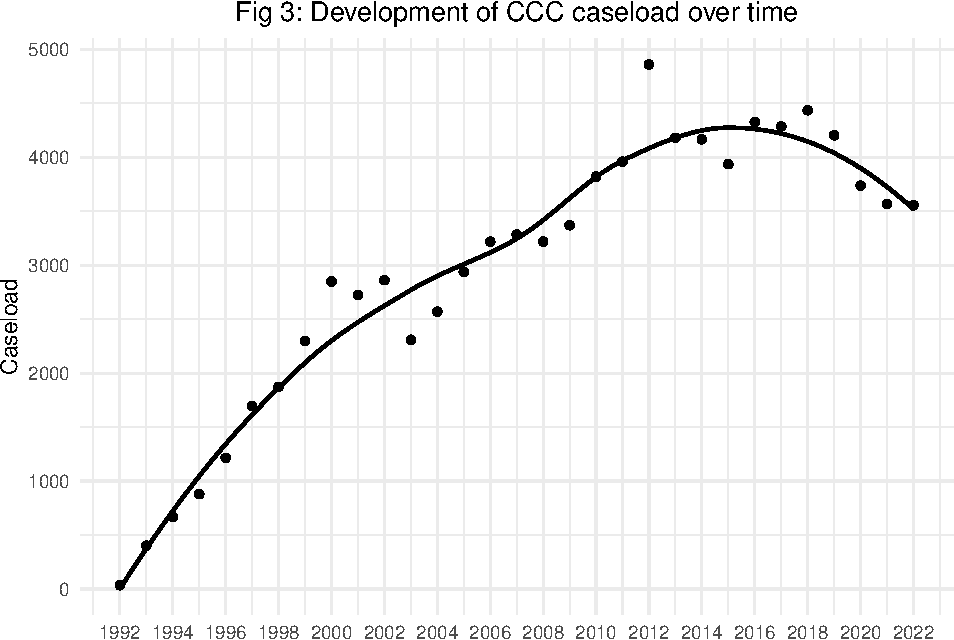
\includegraphics{dissents_article-anonymised_files/figure-latex/caseload_over_time-1.pdf}
We opt for the Bayesian logistic regression model because the dependent
variable is a binomial variable with 1 trial, i.e.~our \emph{Y}, the
decision to dissent or not to dissent of a judge in any given decision:

\[
Y | \pi \sim Bern(\pi)
\] Our model looks as follows:

\[
P(dissent) = f(unfinished\:cases)
\]

\hypertarget{result}{%
\subsubsection{Result}\label{result}}

\hypertarget{interpreting-the-posterior}{%
\paragraph{Interpreting the
posterior}\label{interpreting-the-posterior}}

We observe that the estimate of the workload parameter significantly
differs from 0, as the 95 \% and 80 \% uncertainty intervals of the
posterior draws of the parameter lay on the left of 0. We're thus able
to proceed with substantive interpretation of the result.

\vspace{10pt}

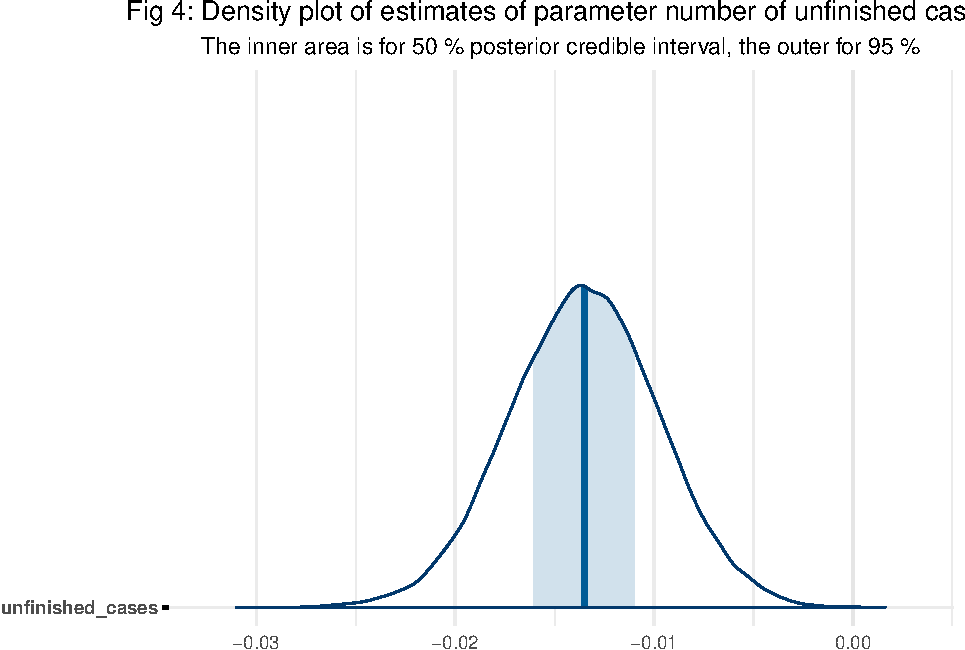
\includegraphics{dissents_article-anonymised_files/figure-latex/interpreting_posterior2-1.pdf}

The regression table is already transformed into odds from the log odds
output of the model. At first glance, the results are in line with our
theoretical predictions.

\begin{longtable}[]{@{}lrrrr@{}}
\toprule\noalign{}
term & estimate\_odds & std.error & conf.low & conf.high \\
\midrule\noalign{}
\endhead
\bottomrule\noalign{}
\endlastfoot
(Intercept) & 0.059 & 1.061 & 0.054 & 0.063 \\
unfinished\_cases & 0.987 & 1.004 & 0.982 & 0.991 \\
\end{longtable}

We observe that for each increase of unfinished cases of a judge in any
decision, the outcome likelihood of dissent decreases by
\textasciitilde0.13 \% (\emph{e}\textsuperscript{-0.0135}). Because the
number of unfinished cases is usually in 10\^{}1 dimensions, the effect
isn't unsubstantial. The result from our analysis is in line with our
intuition. The CCC judges take into account the effort costs of dissent
and square it against their perceived workload. If they are overloaded
with work, the probability that they will dissent in any given case
decreases.

\hypertarget{h3-collegiality-costs-of-dissenting-at-the-ccc}{%
\subsection{\texorpdfstring{H\textsubscript{3}: Collegiality costs of
dissenting at the
CCC}{H3: Collegiality costs of dissenting at the CCC}}\label{h3-collegiality-costs-of-dissenting-at-the-ccc}}

\hypertarget{model-specification-2}{%
\subsubsection{Model specification}\label{model-specification-2}}

We build on our previous model. We now know that the number of dissents
of a judge rapporteur follows a Poisson distribution. We use a
hierarchical model pooled on the judges. We have no knowledge whatsoever
about the effect of start or end of term on the number of dissents,
thus, we use only weakly informative priors. We have addressed the
potential sources of bias with the workload as an explanatory variable
above.

\[
N_{dissents} = f(start\:term + end\:term)
\]

Because of the introduction of the system of bi-yearly rotations of the
3-member panels in 2016, we include in our analysis only the plenary
decisions, where the composition remained relatively stable throughout
the judges' terms.

\hypertarget{results-1}{%
\subsubsection{Results}\label{results-1}}

Unfortunately, neither of the relevant parameters differs significantly
from zero. Therefore, we're unable able to draw any inferential
conclusions from our model.

\vspace{10pt}

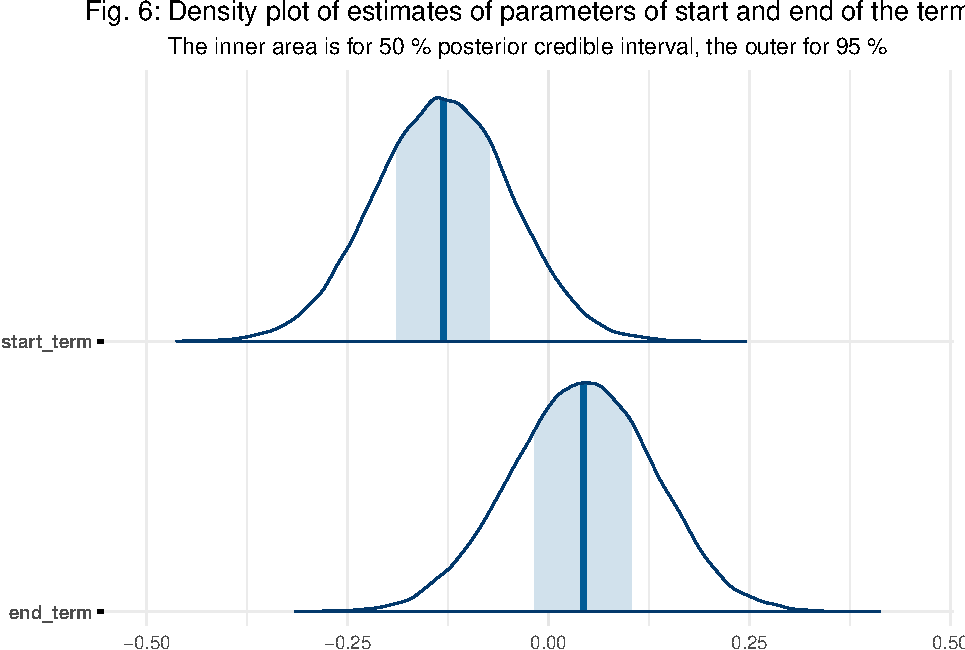
\includegraphics{dissents_article-anonymised_files/figure-latex/interpreting_posterior_term2-1.pdf}

Even if we attempted to interpret the results, the results would be
consistent with the original. The model reveals the trend that the
judges seem to change their dissenting behavior depending on in which
phase of their term do they find themselves, they would be more likely
to dissent at the end and less likely at the beginning of their terms.

\begin{longtable}[]{@{}lrrrr@{}}
\toprule\noalign{}
term & estimate & std.error & conf.low & conf.high \\
\midrule\noalign{}
\endhead
\bottomrule\noalign{}
\endlastfoot
(Intercept) & 2.48 & 1.09 & 2.21 & 2.76 \\
end\_term & 1.04 & 1.09 & 0.93 & 1.17 \\
start\_term & 0.88 & 1.09 & 0.79 & 0.98 \\
\end{longtable}

\hypertarget{h4-judicial-coalitions-formed-in-the-plenary-proceedings-affect-judges-likelihood-to-dissent-in-3-member-panels}{%
\subsection{\texorpdfstring{H\textsubscript{4}: Judicial coalitions
formed in the plenary proceedings affect judges' likelihood to dissent
in 3-member
panels}{H4: Judicial coalitions formed in the plenary proceedings affect judges' likelihood to dissent in 3-member panels}}\label{h4-judicial-coalitions-formed-in-the-plenary-proceedings-affect-judges-likelihood-to-dissent-in-3-member-panels}}

Lastly, we measure the impact of coalitions that formed in the plenary
proceedings on the behavior of judges on the dissenting behavior of
judges. \#\#\# Model specification Practically speaking, we mined the
compositions of panels from the text of the decision in each and every
decision. Following Chmel and Vartazaryan, we split the 3rd term CCC
into two coalitions: the first coalition consisted of judges Kateřina
Šimáčková, Vojtěch Šimíček, Ludvík David, Jaromír Jirsa, David Uhlíř,
Jiří Zemánek, Tomáš Lichovník, Jan Filip, Milada Tomková and Pavel
Šámal, whereas the second coalition of judges consisted of Radovan
Suchánek, Vladimír Sládeček, Josef Fiala, Jan Musil, Jaroslav Fenyk, and
Pavel Rychetský.

We filtered the 3-member panel on merits decisions\footnote{At the
  3-member panel level, procedural decisions have to be unanimous.
  Therefore, they do not leave any variation of dissenting behavior and
  we leave them out of the model.} of the 3rd term CCC and coded the
following dummy variables. One dummy for each coalition, if all 3
members of the panel in any given decision were members of the same
coalition. On top of that, our model included one dummy variable, if one
member of the panel in the minority came from the other coalition of the
2 majority judges.

\[
P(dissent) = f(full\:coalition\:1 + full\:coalition\:2 + mixed\:1\:minority + mixed\:2\:minority)
\]

The assignment to panels is as good as random, thus, there is no need to
control for other covariates. Because our outcome of interest, the
presence of a dissent in any given decision, is a binary variable, we
opted for the binomial logistic regression model. For the model, we used
weakly informative priors as we have no idea about the potential effect
of having the two coalitions.

\hypertarget{results-2}{%
\subsubsection{Results}\label{results-2}}

The regression table is already transformed into odds from the log odds
output of the model.

\begin{longtable}[]{@{}lrrrr@{}}
\toprule\noalign{}
term & estimate\_odds & std.error & conf.low & conf.high \\
\midrule\noalign{}
\endhead
\bottomrule\noalign{}
\endlastfoot
(Intercept) & 0.03 & 21.44 & 0.00 & 1.75 \\
full\_coal\_1 & 0.68 & 21.60 & 0.01 & 32.89 \\
full\_coal\_2 & 0.00 & 2577638.25 & 0.00 & 0.05 \\
mixed\_coal\_1\_min & 2.03 & 21.58 & 0.04 & 99.94 \\
mixed\_coal\_2\_min & 2.12 & 21.35 & 0.04 & 104.20 \\
\end{longtable}

The estimated odds of dissent are already pretty low, the predicted
likelihood of dissent appearing in any 3-member panel decision on merits
is \textasciitilde3 \% (which isn't at odds with our workload model,
where the pool of considered decisions is slightly wider). In our data,
there is not a single dissent among a panel composed of completely of
members from the second coalition, which explains the 0. On the other
hand, the full presence of the first coalition decreases the odds of
dissent considerably by \textasciitilde20 \%. Lastly, the effects of
having both panels mixed are in either case positive, the odds of both
parameters are \textasciitilde2.

\vspace{10pt}

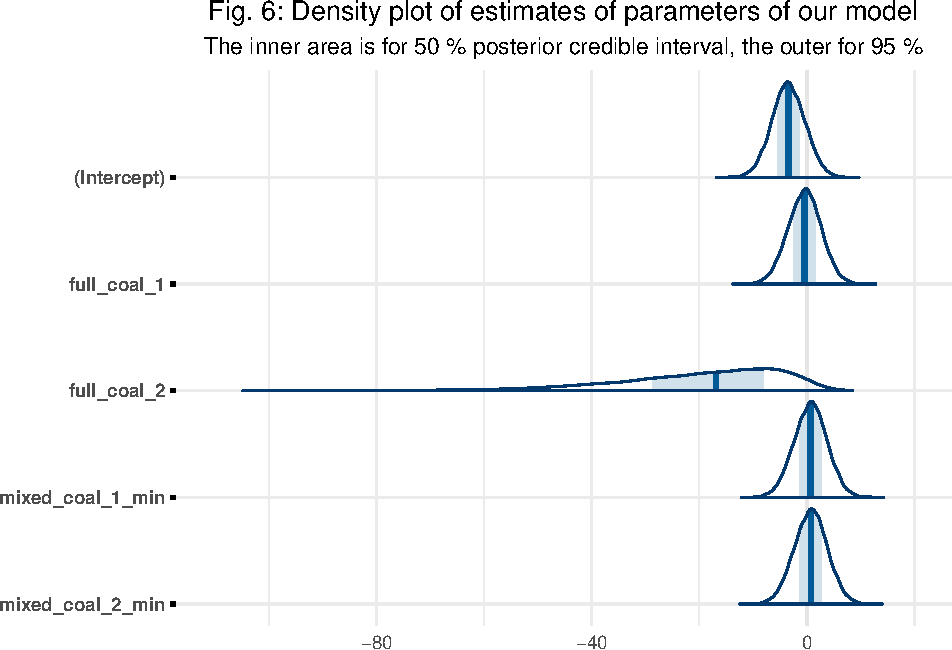
\includegraphics{dissents_article-anonymised_files/figure-latex/interval_coalition-1.pdf}

Interpreting the repercussions for theory is quite difficult, especially
given the lack of data on the second and given the rather large standard
errors. While we steer clear of using the language of causal
relationship, the trend is clear: a panel composed of members from both
coalitions from the plenary proceedings increases the disagreement on
the bench. We could not confirm any heterogenous effects between the two
coalitions. We also cannot exactly pin point the mechanism of the
effect: Do the relationships from the plenary proceedings subsequently
carry over to the 3-member panel proceedings? Is there a 2-way effect?
We thus conclude rather cautiously that our data and evidence seems
reasonably compatible with the explanation of Czech legal scholars,
however, due to large standard errors, the evidence remains
inconclusive.

\hypertarget{conclusions}{%
\section{Conclusions}\label{conclusions}}

We attempted to transplant a research design from the US context to the
European context. We had to adjust it to the extent that data
availability precluded us for posing certain hypotheses or applying
certain methods. Our results are inconclusive as to the potential to
transfer conclusions from empirical legal research conducted in the US
context elsewhere. We believe our study opens up new doors for empirical
legal research, both substantively and methodologically.

Regarding the latter, the method, the prerequisite for our study was
building a large dataset on the Czech Apex Court, which is to be
published soon. Having a large text corpus as well as metadata and
handcoded information about the judges at hand unlocks a lot of new
potential research avenues, including research utilizing quantative text
analysis, machine learning etc.

We're very well aware that, on the one hand, utilizing, for example,
machine learning to process large amount of court decisions in itself
solves all the issues, we're also aware that it introduces new
uncertainties and inaccuracies. On the other hand, it allowed us to
conduct an empirical research in an environment, in which it has not
traditionally been conducted.

Our next remark addresses our research design in general: the regression
analysis. We are aware that given the potential outcome frameworks, it
is difficult to sustain all the assumptions of regression research
design. Experimental or quasi-experimental research design such as
difference-in-differences or discontinuity designs should be the golden
standard of social science (Bueno de Mesquita and Fowler 2021). The
relative unmalleability of law in general, but rather conservative
institutions such as courts in particular, leaves little space for
experimental design and the general applicability of law within a legal
system leaves little space for quasi-experimental design. That is not to
say that it is impossible. Although we tried our best to think of and to
address all potential sources of bias and whether the assumptions of the
models of choice were met, we are aware of limitations of
regression-based research design and therefore our conclusions should be
taken with a grain of salt.

Regarding the substantive results, to us a little surprisingly, we
reached very similar results as the Epstein, Landes, and Posner (2011)
study. We found that a dissent opinion imposes costs on the majority
that produces longer arguments to address a dissent. The effect is
stronger the more disagreement there is on the bench. We find that the
workload of a judge does decrease the likelihood of dissent. Moreover,
although inconclusively, the dissenting behavior of a CCC judge seems to
vary depending on the stage of their term. Lastly, we reveal similar
trends in behavior of judicial coalitions from plenary proceedings also
in the 3-member panel proceedings.

We believe those to be very interesting findings that can be further
developed. While we found some clear trends, it is uncertain whether our
explanation always fits the data perfectly as there are always plausible
competing explanations. To this end we believe that a qualitative study
utilizing interviews could shed more light to our substantive
findings.\footnote{Which we are currently working on.}

\vspace{30pt}

\hypertarget{literature}{%
\section*{Literature}\label{literature}}
\addcontentsline{toc}{section}{Literature}

\hypertarget{refs}{}
\begin{CSLReferences}{1}{0}
\leavevmode\vadjust pre{\hypertarget{ref-angristMasteringMetricsPath2015}{}}%
Angrist, Joshua David, and Jörn-Steffen Pischke. 2015. \emph{Mastering
'Metrics: The Path from Cause to Effect}. {Princeton ; Oxford}:
{Princeton University Press}.

\leavevmode\vadjust pre{\hypertarget{ref-angristMostlyHarmlessEconometrics2009}{}}%
Angrist, Joshua D., and Jörn-Steffen Pischke. 2009. \emph{Mostly
{Harmless Econometrics}: {An Empiricist}'s {Companion}}. {Princeton
University Press}. \url{https://books.google.com?id=YSAzEAAAQBAJ}.

\leavevmode\vadjust pre{\hypertarget{ref-berdejoElectoralCyclesUS2017}{}}%
Berdejó, Carlos, and Daniel L. Chen. 2017. {``Electoral {Cycles} Among
{US Courts} of {Appeals Judges}.''} \emph{The Journal of Law and
Economics} 60 (3): 479--96. \url{https://doi.org/10.1086/696237}.

\leavevmode\vadjust pre{\hypertarget{ref-boydUntanglingCausalEffects2010}{}}%
Boyd, Christina L., Lee Epstein, and Andrew D. Martin. 2010.
{``Untangling the {Causal Effects} of {Sex} on {Judging}.''}
\emph{American Journal of Political Science} 54 (2): 389--411.
\url{https://www.jstor.org/stable/25652213}.

\leavevmode\vadjust pre{\hypertarget{ref-brekkeCJEUDatabasePlatform2023}{}}%
Brekke, Stein Arne, Joshua C. Fjelstul, Silje Synnøve Lyder Hermansen,
and Daniel Naurin. 2023. {``The {CJEU Database Platform}: {Decisions}
and {Decision-Makers}.''} \emph{Journal of Law and Courts}, January,
1--22. \url{https://doi.org/10.1017/jlc.2022.3}.

\leavevmode\vadjust pre{\hypertarget{ref-buenodemesquitaThinkingClearlyData2021}{}}%
Bueno de Mesquita, Ethan, and Anthony Fowler, eds. 2021. \emph{Thinking
Clearly with Data: A Guide to Quantitative Reasoning and Analysis}. 1st.
edition. {Princeton}: {Princeton University Press}.

\leavevmode\vadjust pre{\hypertarget{ref-carrubbaWhoControlsContent2012}{}}%
Carrubba, Cliff, Barry Friedman, Andrew D. Martin, and Georg Vanberg.
2012. {``Who {Controls} the {Content} of {Supreme Court Opinions}?''}
\emph{American Journal of Political Science} 56 (2): 400--412.
\url{https://doi.org/10.1111/j.1540-5907.2011.00557.x}.

\leavevmode\vadjust pre{\hypertarget{ref-chmelCoOvlivnujeUstavni2021}{}}%
Chmel, Jan. 2021. \emph{Co Ovlivňuje {Ústavní} Soud a Jeho Soudce? /}.
Vydání první. Teoretik ({Leges}). {Leges,}.

\leavevmode\vadjust pre{\hypertarget{ref-clarkLocatingSupremeCourt2010}{}}%
Clark, Tom S., and Benjamin Lauderdale. 2010. {``Locating {Supreme Court
Opinions} in {Doctrine Space}.''} \emph{American Journal of Political
Science} 54 (4): 871--90.
\url{https://doi.org/10.1111/j.1540-5907.2010.00470.x}.

\leavevmode\vadjust pre{\hypertarget{ref-dworkinPoliticalJudgesRule1980}{}}%
Dworkin, Ronald M. 1980. \emph{Political Judges and the Rule of Law}.
{London}: {British Academy}.

\leavevmode\vadjust pre{\hypertarget{ref-eliasekAutomatickaKlasifikaceVyznamovych2020}{}}%
Eliášek, Martin, Jakub Kól, and Miloš Švaňa. 2020. {``Automatická
Klasifikace Významových Celků v Judikatuře.''} \emph{Revue Pro Právo a
Technologie} 11 (21): 3--20. \url{https://doi.org/10.5817/RPT2020-1-1}.

\leavevmode\vadjust pre{\hypertarget{ref-epsteinStrategicRevolutionJudicial2000}{}}%
Epstein, Lee, and Jack Knight. 2000. {``Toward a {Strategic Revolution}
in {Judicial Politics}: {A Look Back}, {A Look Ahead}.''}
\emph{Political Research Quarterly} 53 (3): 625--61.
\url{https://doi.org/10.1177/106591290005300309}.

\leavevmode\vadjust pre{\hypertarget{ref-epsteinWhyWhenJudges2011}{}}%
Epstein, Lee, William M. Landes, and Richard A. Posner. 2011. {``Why
({And When}) {Judges Dissent}: {A Theoretical And Empirical
Analysis}.''} \emph{Journal of Legal Analysis} 3 (1): 101--37.
\url{https://doi.org/10.1093/jla/3.1.101}.

\leavevmode\vadjust pre{\hypertarget{ref-fjelstulHowChamberSystem2021}{}}%
Fjelstul, Joshua. 2021. {``How the {Chamber System} at the {CJEU
Undermines} the {Consistency} of the {Court}'s {Application} of {EU
Law}.''} \emph{Journal of Law and Courts}, November, 717422.
\url{https://doi.org/10.1086/717422}.

\leavevmode\vadjust pre{\hypertarget{ref-foxallWhatJudgesMaximize2004}{}}%
Foxall, Gordon R. 2004. {``What Judges Maximize:toward an Economic
Psychology of the Judicial Utility Function.''} \emph{Liverpool Law
Review} 25 (3): 177--94.
\url{https://doi.org/10.1007/s10991-004-2877-9}.

\leavevmode\vadjust pre{\hypertarget{ref-gandhiSupportVectorMachine2018}{}}%
Gandhi, Rohith. 2018. {``Support {Vector Machine} --- {Introduction} to
{Machine Learning Algorithms}.''} {Towards Data Science}. July 5, 2018.
\url{https://towardsdatascience.com/support-vector-machine-introduction-to-machine-learning-algorithms-934a444fca47}.

\leavevmode\vadjust pre{\hypertarget{ref-harastaAutomaticSegmentationCzech2019}{}}%
Harašta, Jakub, Jaromír Šavelka, František Kasl, and Jakub Míšek. 2019.
{``Automatic {Segmentation} of {Czech Court Decisions} into
{Multi-Paragraph Parts}.''} \emph{Jusletter IT} 4 (M).
\url{https://is.muni.cz/publication/1534440/cs/Automatic-Segmentation-of-Czech-Court-Decisions-into-Multi-Paragraph-Parts/Harasta-Savelka-Kasl-Misek}.

\leavevmode\vadjust pre{\hypertarget{ref-hyndmanTransformingDataZeros2010}{}}%
Hyndman, Rob. 2010. {``Transforming Data with Zeros.''} {Rob Hyndman}.
August 13, 2010.
\url{https://robjhyndman.com/hyndsight/transformations/}.

\leavevmode\vadjust pre{\hypertarget{ref-kastellecEmpiricallyEvaluatingCountermajoritarian2016}{}}%
Kastellec, Jonathan P. 2016. {``Empirically {Evaluating} the
{Countermajoritarian Difficulty}: {Public Opinion}, {State Policy}, and
{Judicial Review} Before {\emph{Roe}}{ \emph{v.} }{\emph{Wade}}.''}
\emph{Journal of Law and Courts} 4 (1): 1--42.
\url{https://doi.org/10.1086/683466}.

\leavevmode\vadjust pre{\hypertarget{ref-ludersProportionalityArgumentIdentification2023}{}}%
Lüders, Kilian, and Bent Stohlman. 2023. {``Proportionality as an
Argument: {Identification} of a Judicial Decision Technique.''}
\emph{DRAFT for 5th ANNUAL COMPTEXT Conference}.

\leavevmode\vadjust pre{\hypertarget{ref-maklinGradientBoostingDecision2019}{}}%
Maklin, Cory. 2019. {``Gradient {Boosting Decision Tree Algorithm
Explained}.''} {Towards Data Science}. July 21, 2019.
\url{https://towardsdatascience.com/machine-learning-part-18-boosting-algorithms-gradient-boosting-in-python-ef5ae6965be4}.

\leavevmode\vadjust pre{\hypertarget{ref-mikolovEfficientEstimationWord2013}{}}%
Mikolov, Tomas, Kai Chen, Greg Corrado, and Jeffrey Dean. 2013.
{``Efficient {Estimation} of {Word Representations} in {Vector
Space}.''} September 6, 2013.
\url{https://doi.org/10.48550/arXiv.1301.3781}.

\leavevmode\vadjust pre{\hypertarget{ref-montgomeryHowConditioningPosttreatment2018}{}}%
Montgomery, Jacob M., Brendan Nyhan, and Michelle Torres. 2018. {``How
{Conditioning} on {Posttreatment Variables Can Ruin Your Experiment} and
{What} to {Do} about {It}.''} \emph{American Journal of Political
Science} 62 (3): 760--75. \url{https://www.jstor.org/stable/26598780}.

\leavevmode\vadjust pre{\hypertarget{ref-moyerJudicialInnovationSexual2012}{}}%
Moyer, Laura P., and Holley Tankersley. 2012. {``Judicial {Innovation}
and {Sexual Harassment Doctrine} in the {U}.{S}. {Courts} of
{Appeals}.''} \emph{Political Research Quarterly} 65 (4): 784--98.
\url{https://doi.org/10.1177/1065912911411097}.

\leavevmode\vadjust pre{\hypertarget{ref-posnerWhatJudgesJustices1993}{}}%
Posner, Richard A. 1993. \emph{What {Do Judges} and {Justices
Maximize}?: (The {Same Thing Everyone Else Does})}. {Law School,
University of Chicago}. \url{https://books.google.com?id=ciFUHQAACAAJ}.

\leavevmode\vadjust pre{\hypertarget{ref-posnerHowJudgesThink2010}{}}%
---------. 2010. \emph{How {Judges Think}}. {Harvard University Press}.
\url{https://books.google.com?id=ZVUC8riEVPQC}.

\leavevmode\vadjust pre{\hypertarget{ref-segalIdeologicalValuesVotes1995}{}}%
Segal, Jeffrey A., Lee Epstein, Charles M. Cameron, and Harold J.
Spaeth. 1995. {``Ideological {Values} and the {Votes} of {U}.{S}.
{Supreme Court Justices Revisited}.''} \emph{The Journal of Politics} 57
(3): 812--23. \url{https://doi.org/10.2307/2960194}.

\leavevmode\vadjust pre{\hypertarget{ref-smekalMimopravniVlivyNa2021}{}}%
Smekal, Hubert, Jaroslav Benák, Monika Hanych, Ladislav Vyhnánek, and
Štěpán Janků. 2021. \emph{Mimoprávní Vlivy Na Rozhodování Českého
{Ústavního} Soudu:} {Brno}: {Masaryk University Press}.
\url{https://doi.org/10.5817/CZ.MUNI.M210-9884-2021}.

\leavevmode\vadjust pre{\hypertarget{ref-vartazaryanSitOvaAnalyza2022}{}}%
Vartazaryan, Gor. 2022. {``Sít'ová Analỳza Disentujících Ústavních
Soudců.''} \emph{Pravnik}, no. 12.

\end{CSLReferences}

\end{document}
